%\documentclass[icelandic]{beamer}

\documentclass[icelandic,a4paper,12pt]{article}
\usepackage{beamerarticle}

\mode<presentation>
{
  \usetheme{boxes}
  % með efnisyfirliti: Szeged, Frankfurt 
  % án efnisyfirlits: Pittsburgh
  % áhugavert: CambridgeUS, Boadilla
  %\setbeamercovered{transparent} %gegnsætt
  \setbeamercovered{invisible}
  }

\usepackage[english,icelandic]{babel}
\usepackage[utf8]{inputenc}
\usepackage{t1enc}
\selectlanguage{icelandic}
\usepackage{graphicx}
\usepackage{amsmath}
\usepackage{amssymb}
\usepackage{mathrsfs}
% \newcommand{\C}{{\mathbb  C}}
% \newcommand{\Z}{{\mathbb Z}}
% \newcommand{\R}{{\mathbb  R}}
% \newcommand{\N}{{\mathbb  N}}
% \newcommand{\Q}{{\mathbb Q}}
\renewcommand{\phi}{\varphi}
\renewcommand{\epsilon}{\varepsilon}

%\usepackage{pgfpages}
% \pgfpagesuselayout{2 on 1}[a4paper,border shrink=5mm]

\def\lecturename{Stærðfræðigreining IB}
\title{\insertlecture}
\author{Benedikt Steinar Magnússon, \href{mailto:bsm@hi.is}{bsm@hi.is}}
\institute
{
  Verkfræði- og náttúruvísindasvið\\
  Háskóli Íslands
}
\subtitle{Stærðfræðigreining IB}
%\subject{\lecturename}

\mode<article>
{
	\usepackage[colorlinks=false,
	pdfauthor={Benedikt Steinar Magnusson},
	pdftitle={IB: Namsefni
	}]{hyperref}
  %\usepackage{times}
  %\usepackage{mathptmx}
  \usepackage[left=1.5cm,right=4cm,top=1.5cm,bottom=3cm]{geometry}
}

% Beamer version theme settings

%\useoutertheme[height=0pt,width=2cm,right]{sidebar}
%\usecolortheme{rose,sidebartab}
%\useinnertheme{circles}
%\usefonttheme[only large]{structurebold}

\setbeamercolor{sidebar right}{bg=black!15}
\setbeamercolor{structure}{fg=blue}
\setbeamercolor{author}{parent=structure}

\setbeamerfont{title}{series=\normalfont,size=\LARGE}
\setbeamerfont{title in sidebar}{series=\bfseries}
\setbeamerfont{author in sidebar}{series=\bfseries}
\setbeamerfont*{item}{series=}
\setbeamerfont{frametitle}{size=}
\setbeamerfont{block title}{size=\small}
\setbeamerfont{subtitle}{size=\normalsize,series=\normalfont}

\defbeamertemplate*{footline}{infolines theme}
 {
   \leavevmode%
   \hbox{%
   \begin{beamercolorbox}[wd=.333333\paperwidth,ht=2.25ex,dp=1ex,center]{author in head/foot}%
   %  \usebeamerfont{author in head/foot}\insertshortauthor~~\beamer@ifempty{\insertshortinstitute}{}{(\insertshortinstitute)}
   \end{beamercolorbox}%
   \begin{beamercolorbox}[wd=.333333\paperwidth,ht=2.25ex,dp=1ex,center]{title in head/foot}%
    % \usebeamerfont{title in head/foot}\insertshorttitle
   \end{beamercolorbox}%
   \begin{beamercolorbox}[wd=.333333\paperwidth,ht=2.25ex,dp=1ex,right]{date in head/foot}%
     %\usebeamerfont{date in head/foot}\insertshortdate{}\hspace*{2em}
     \insertshortlecture.\insertframenumber{} / \insertshortlecture.\inserttotalframenumber\hspace*{2ex} 
   \end{beamercolorbox}}%
   \vskip0pt%
 }
  


\setbeamertemplate{sidebar right}
{
  {\usebeamerfont{title in sidebar}%
    \vskip1.5em%
    \hskip3pt%
    \usebeamercolor[fg]{title in sidebar}%
    \insertshorttitle[width=2cm-6pt,center,respectlinebreaks]\par%
    \vskip1.25em%
  }%
  {%
    \hskip3pt%
    \usebeamercolor[fg]{author in sidebar}%
    \usebeamerfont{author in sidebar}%
    \insertshortauthor[width=2cm-2pt,center,respectlinebreaks]\par%
    \vskip1.25em%
  }%
  \hbox to2cm{\hss\insertlogo\hss}
  \vskip1.25em%
  \insertverticalnavigation{2cm}%
  \vfill
  \hbox to 2cm{\hfill\usebeamerfont{subsection in
      sidebar}\strut\usebeamercolor[fg]{subsection in
      sidebar}\insertshortlecture.\insertframenumber\hskip5pt}%
  \vskip3pt%
}%

\setbeamertemplate{title page}
{
  \vbox{}
  \vskip1em
  %{\huge Kapitel \insertshortlecture\par}
  {\usebeamercolor[fg]{title}\usebeamerfont{title}\inserttitle\par}%
  \ifx\insertsubtitle\@empty%
  \else%
    \vskip0.25em%
    {\usebeamerfont{subtitle}\usebeamercolor[fg]{subtitle}\insertsubtitle\par}%
  \fi%     
  \vskip1em\par
  %Vorlesung \emph{\lecturename}\ vom 
  \insertdate\par
  \vskip0pt plus1filll
  \leftskip=0pt plus1fill\insertauthor\par
  \insertinstitute\vskip1em
}

%\logo{\includegraphics[width=2cm]{beamerexample-lecture-logo.pdf}}



% Article version layout settings

\mode<article>

\makeatletter
\def\@listI{\leftmargin\leftmargini
  \parsep 0pt
  \topsep 5\p@   \@plus3\p@ \@minus5\p@
  \itemsep0pt}
\let\@listi=\@listI


\setbeamertemplate{frametitle}{\paragraph*{\insertframetitle\
    \ \small\insertframesubtitle}\ \par
}
\setbeamertemplate{frame end}{%
  \marginpar{\scriptsize\hbox to 1cm{\sffamily%
      \hfill\strut\insertshortlecture.\insertframenumber}\hrule height .2pt}}
\setlength{\marginparwidth}{1cm}
\setlength{\marginparsep}{1.5cm}

\def\@maketitle{\makechapter}

\def\makechapter{
  \newpage
  \null
  \vskip 2em%
  {%
    \parindent=0pt
    \raggedright
    \sffamily
    \vskip8pt
    %{\fontsize{36pt}{36pt}\selectfont Kapitel \insertshortlecture \par\vskip2pt}
    {\fontsize{24pt}{28pt}\selectfont \color{blue!50!black} \insertlecture\par\vskip4pt}
    {\Large\selectfont \color{blue!50!black} \insertsubtitle, \@date\par}
    \vskip10pt

    \normalsize\selectfont \@author\par\vskip1.5em
    %\hfill BLABLA
  }
  \par
  \vskip 1.5em%
}

\let\origstartsection=\@startsection
\def\@startsection#1#2#3#4#5#6{%
  \origstartsection{#1}{#2}{#3}{#4}{#5}{#6\normalfont\sffamily\color{blue!50!black}\selectfont}}

\makeatother

\mode
<all>




% Typesetting Listings

\usepackage{listings}
\lstset{language=Java}

\alt<presentation>
{\lstset{%
  basicstyle=\footnotesize\ttfamily,
  commentstyle=\slshape\color{green!50!black},
  keywordstyle=\bfseries\color{blue!50!black},
  identifierstyle=\color{blue},
  stringstyle=\color{orange},
  escapechar=\#,
  emphstyle=\color{red}}
}
{
  \lstset{%
    basicstyle=\ttfamily,
    keywordstyle=\bfseries,
    commentstyle=\itshape,
    escapechar=\#,
    emphstyle=\bfseries\color{red}
  }
}



% Common theorem-like environments

\theoremstyle{definition}
\newtheorem{exercise}[theorem]{\translate{Exercise}}




% New useful definitions:

\newbox\mytempbox
\newdimen\mytempdimen

\newcommand\includegraphicscopyright[3][]{%
  \leavevmode\vbox{\vskip3pt\raggedright\setbox\mytempbox=\hbox{\includegraphics[#1]{#2}}%
    \mytempdimen=\wd\mytempbox\box\mytempbox\par\vskip1pt%
    \fontsize{3}{3.5}\selectfont{\color{black!25}{\vbox{\hsize=\mytempdimen#3}}}\vskip3pt%
}}

\newenvironment{colortabular}[1]{\medskip\rowcolors[]{1}{blue!20}{blue!10}\tabular{#1}\rowcolor{blue!40}}{\endtabular\medskip}

\def\equad{\leavevmode\hbox{}\quad}

\newenvironment{greencolortabular}[1]
{\medskip\rowcolors[]{1}{green!50!black!20}{green!50!black!10}%
  \tabular{#1}\rowcolor{green!50!black!40}}%
{\endtabular\medskip}



\lecture[1]{2. Markgildi og samfelldni}{lecture-text}
\date{29. ágúst 2015}

\newcommand{\C}{{\mathbb  C}}
\newcommand{\Z}{{\mathbb Z}}
\newcommand{\R}{{\mathbb  R}}
\newcommand{\N}{{\mathbb  N}}
\newcommand{\Q}{{\mathbb Q}}
\newcommand{\Sin}{{\text{Sin}}}
\newcommand{\Tan}{{\text{Tan}}}
\newcommand{\Cos}{{\text{Cos}}}
\newcommand{\Cosh}{{\text{Cosh}}}
\newcommand{\arsinh}{{\text{arsinh}}}
\newcommand{\arcosh}{{\text{arcosh}}}
\newcommand{\artanh}{{\text{artanh}}}


\begin{document}
\setcounter{tocdepth}{2}
\tableofcontents

\section{Heildun}
\subsection{Heildun jákvæðra falla}
\subsubsection{Skilgreining: Heildi}   
Látum $f:[a,b]\rightarrow \R$ 
vera fall þannig að $f(x)\geq 0$ fyrir öll
$x\in[a,b]$.  

Þegar heildið $\int_a^b f(x)\,dx$ er skilgreint er útkoman úr
því flatarmál svæðisins sem liggur á milli $x$-ás og grafs fallsins
(og afmarkast til vinstri af línunni $x=a$ og til hægri af línunni
$x=b$).   

Ef heildið  $\int_a^b f(x)\,dx$ er skilgreint þá segjum við
að fallið $f$ sé \emph{heildanlegt} yfir bilið $[a,b]$. 

Tölurnar $a$ og $b$ kallast \emph{heildismörk} heildisins.

\subsubsection{Skilgreining}   
Látum $f$ vera fall.  
Skilgreinum föllin $f_+$
og $f_-$, sem bæði hafa sama skilgreiningarsvæði og $f$, með
$$
  f_+(x)=\left\{\begin{array}{ll} f(x) & \mbox{ef }f(x)\geq 0,\\
  0 & \mbox{ef }f(x)<0, \end{array} \right. \qquad
  f_-(x)=\left\{\begin{array}{ll} 0 & \mbox{ef }f(x)\geq 0,\\
  -f(x) & \mbox{ef }f(x)<0. \end{array}\right.
$$

Athugið að $f(x)=f_+(x)-f_-(x)$.

.. todo::
  mynd

\subsubsection{Setning} 
Takmarkað fall $f$ er \emph{heildanlegt} yfir bilið
$[a, b]$ ef bæði föllin $f_+$ og $f_-$ eru heildanleg yfir bilið $[a,
b]$.  Ef fallið $f$ er heildanlegt þá skilgreinum við heildi þess með
formúlunni
$$\int_a^b f(x)\,dx=\int_a^b f_+(x)\,dx-\int_a^b f_-(x)\,dx.$$

.. note::
  Flatarmálið sem er undir $x$-ás reiknast neikvætt.

\subsubsection{Setning}
\begin{enumerate}[(i)]
\item Ef fallið $f$ er samfellt á bilinu $[a, b]$ þá er $f$ heildanlegt yfir bilið $[a, b]$.
\item Einhalla fall skilgreint á bili $[a,b]$ er heildanlegt.
\end{enumerate}
 
\subsubsection{Setning}
Látum $f$ vera fall sem er heildanlegt yfir bilið $[a, b]$. Þá er 
$$
  \Big|\int_a^b f(x)\,dx\Big|\leq \int_a^b |f(x)|\,dx.
$$

\subsection{Eiginleikar heildisins}

\subsubsection{Skilgreining: Heildismörkunum snúið við} 
Ef fallið $f$ er heildanlegt yfir bilið $[a,b]$ (hér er $a<b$) þá skilgreinum við 
$$\int_b^a f(x)\,dx=-\int_a^b f(x)\,dx.$$

\subsubsection{Setning}  
\begin{enumerate}[(i)]
\item $\int_a^a f(x)\,dx=0$. 
\item $\int_a^b f(x)\,dx=\int_a^c f(x)\,dx+\int_c^b f(x)\,dx$ 

(Hér er náttúrlega forsenda að öll heildin séu skilgreind.)
\end{enumerate}
 
\subsubsection{Setning} 
Látum $f$ og $g$ vera föll sem eru heildanleg yfir bilið $[a,b]$ og látum
$A$ og $B$ vera fasta.  
Þá er $$
  \int_a^b Af(x)+Bg(x)\,dx=A\int_a^b f(x)\,dx+B\int_a^b g(x)\,dx.
$$
 
Með öðrum orðum, heildun er línuleg aðgerð.

\subsubsection{Setning}
Látum $f$ vera fall sem er heildanlegt yfir bilið $[a, b]$.
Gerum ráð fyrir að um öll $x\in [a, b]$ gildi að $f(x)\geq 0$. 
Þá er 
$$
\int_a^b f(x)\,dx\geq 0.
$$

\subsubsection{Fylgisetning}  
\begin{enumerate}[(i)]
\item Látum $f$ og $g$ vera föll sem eru heildanleg yfir bilið $[a, b]$.
Gerum ráð fyrir að um öll $x\in [a, b]$ gildi að $f(x)\leq g(x)$.  Þá  er
$$\int_a^b f(x)\,dx\leq \int_a^b g(x)\,dx.$$
\item Látum $f$ vera fall sem er heildanlegt yfir bilið $[a, b]$. 
Ef $m$ og $M$ eru fastar þannig að um öll $x\in [a, b]$ gildir að $m\leq f(x)\leq M$  
þá er 
$$
m(b-a)= \int_a^b m\,dx \leq  \int_a^b f(x)\,dx \leq \int_a^b M\,dx =M(b-a).
$$
\end{enumerate}

\subsubsection{Setning}  
Látum $f$ vera fall sem er heildanlegt yfir bil $[-a, a]$.
\begin{enumerate}[(i)]
\item Ef fallið $f$ er oddstætt þá er 
$$\int_{-a}^a f(x)\,dx=0.$$
\item Ef fallið $f$ er jafnstætt þá er 
$$\int_{-a}^a f(x)\,dx=2\int_0^a f(x)\,dx.$$
\end{enumerate}

\subsubsection{Skilgreining}
Látum $f$ vera fall sem er heildanlegt yfir bilið $[a, b]$. 
 \emph{Meðalgildi} fallsins $f$ á bilinu $[a, b]$ er skilgreint sem 
$$\bar{f}=\frac{1}{b-a}\int_{a}^b f(x)\,dx.$$

\subsubsection{Setning (Milligildissetning fyrir heildi)}
Gerum ráð fyrir að fallið $f$ sé {\bf samfellt} á bilinu $[a, b]$.  
Þá er til punktur $c$ í bilinu $[a, b]$ þannig að 
$$\int_a^b f(x)\,dx=(b-a)f(c).$$
Það er að segja, til er punktur $c$ í bilinu $[a, b]$ þannig að
$f(c)=\bar{f}$. 

\subsection{Undir- og yfirsummur}
\subsubsection{Dæmi: Að finna heildi}
Hvernig getum við fundið flatarmálið $\int_a^b f(x)\, dx$?

\textbf{Svar}
Við þurfum að nálga flatarmálið með formum sem hafa þekkt
flatarmál, 
til dæmis rétthyrningum.

\subsubsection{Skilgreining}
Skiptum bilinu $[a,b]$ í $n$ parta. Á hverjum parti komum við 
fyrir rétthyrning sem liggur undir grafi fallsins, þ.e. hæðin á 
honum er lággildi fallsins á þessum tiltekna parti. 
\begin{center}
  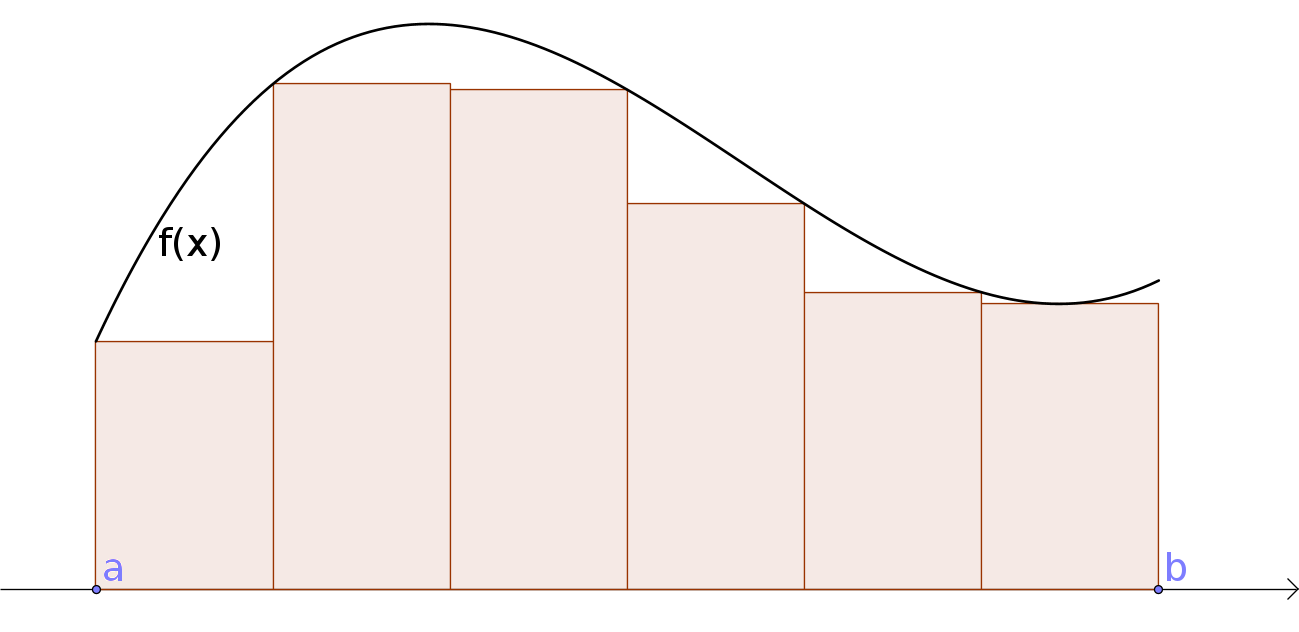
\includegraphics[width=7cm]{./myndir/kafli06/03_undirsumma.png}
\end{center}

Látum $u_k$ vera flatarmál rétthyrninganna, þar sem $k=1,\ldots,n$.

Við köllum flatarmál allra rétthyrninganna \emph{undirsummu} fyrir heildið
og táknum hana með $U(n)$, það er $U(n) = \sum_{k=1}^n u_k$.

Þá er augljóslega $U(n) \leq \int_a^b f(x)\, dx$.

Þegar $n$ stækkar þá fáum við betri og betri nálgun á heildinu.

\subsubsection{Skilgreining}
Skiptum bilinu $[a,b]$ í $n$ parta. Á hverjum parti komum við 
fyrir rétthyrning sem er þannig að  hæðin á 
honum er hágildi fallsins á þessum tiltekna parti. 
\begin{center}
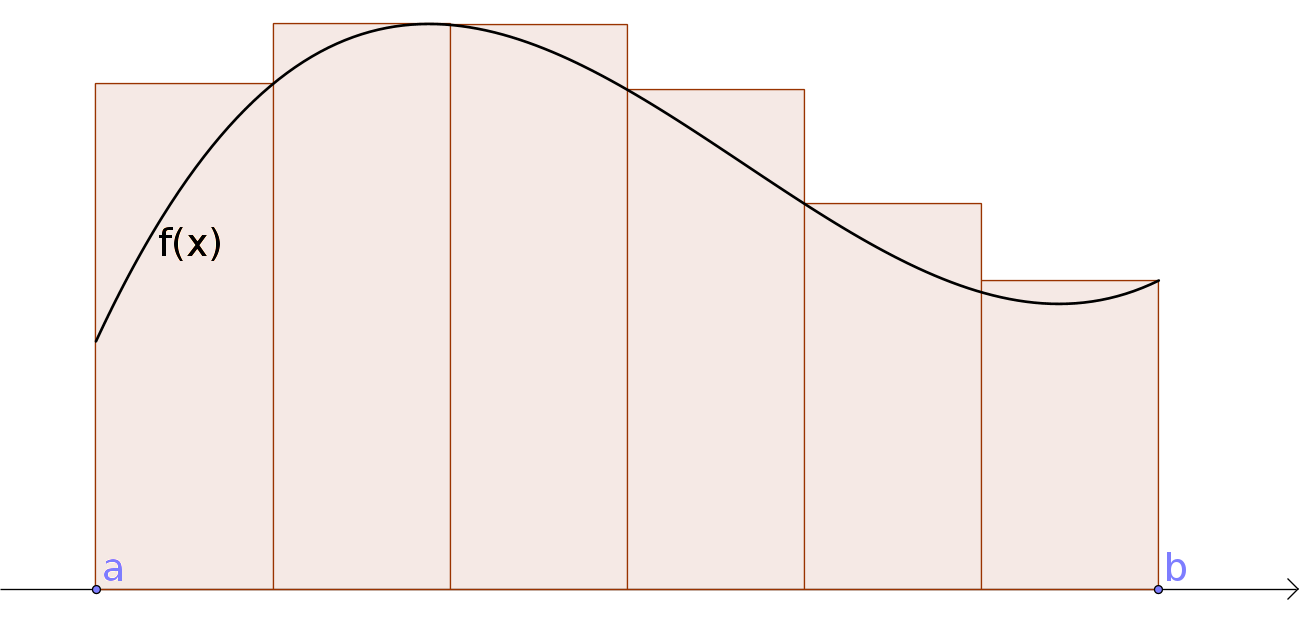
\includegraphics[width=7cm]{./myndir/kafli06/03_yfirsumma.png}
\end{center}
Táknum flatarmál hans með $y_k$, þar sem $k=1,\ldots,n$.
Við köllum summu flatarmáls allra rétthyrninganna \emph{yfirsummu} fyrir heildið
og táknum hana með $Y(n)$, það er $Y(n) = \sum_{k=1}^n y_k$.

Þá fæst að $\int_a^b f(x)\, dx \leq Y(n)$. 

Þegar $n$ stækkar þá fáum við  betri og betri nálgun á heildinu.

\subsubsection{Setning}
Ef til er {\bf nákvæmlega ein} tala $I$ þannig að 
$$
U(n) \leq I \leq Y(n),
$$
fyrir allar undirsummur $U(n)$ og yfirsummur $Y(n)$ þá er fallið
$f$ heildanlegt á $[a,b]$  og 
$$
I = \int_a^b f(x)\, dx.
$$

\subsubsection{Athugasemd}
Við sögðum ekkert um það hvernig við skiptum bilinu $[a,b]$ í $n$ parta. 
Það má gera hvernig sem er, það er ekki nauðsynlegt að þeir séu allir jafn stórir.

\subsubsection{Athugasemd}
Við erum ekki bundin af því að skoða rétthyrninga sem með hæð sem er há/lággildi 
fallsins á hverjum parti, t.d.~má taka miðgildið á hverjum parti,
gildið í hægri endapunkti eða gildið í vinstri endapunkti. 

Niðurstaðan þegar $n\to \infty$ verður hins vegar alltaf sú sama, þ.e.~við nálgumst heildið.

\subsubsection{Athugasemd}
Einnig er mögulegt að nálga heildið með öðrum formum
en rétthyrningum, t.d.~trapisum (sjá kafla 6.6), og
hentar það hugsanlega betur í tölulegum útreikningum.

\subsection{Undirstöðusetning stærðfræðigreiningarinnar}
\subsubsection{Skilgreining og setning: Fall skilgreint með heildi}
Látum $f$ vera fall sem er heildanlegt yfir bil $[a, b]$. 
Fyrir $x\in[a, b]$ skilgreinum við $F(x)=\int_a^x f(t)\,dt$.  Fallið $F$ er
samfellt á $[a, b]$.

\subsubsection{Athugasemd}
Athugið að $t$ er breytan sem er heildað með tilliti til, en
$x$ er haldið föstu á meðan. $t$ hverfur svo þegar búið er að reikna heildið.

\subsubsection{Setning: Undirstöðusetning stærðfræðigreiningar -- fyrri hluti, Theorem~5 Part I, 5.5}
Gerum ráð fyrir að fallið $f$ sé samfellt á bili $I$ og $a$ sé punktur í $I$.  
Fyrir $x$ í $I$ skilgreinum við $F(x)=\int_a^x f(t)\,dt$. Þá er fallið $F$ diffranlegt og 
$$F'(x)=f(x)$$ fyrir öll $x\in I$.

\subsection{Stofnföll}
\subsubsection{Skilgreining} Látum $f$ vera fall sem er skilgreint á bili
$I$.  Fall $G$ kallast \emph{stofnfall} (e. antiderivative) fyrir $f$ á
bilinu $I$ ef $G'(x)=f(x)$ fyrir öll $x$ í $I$.

\subsubsection{Fylgisetning} Látum $f$ vera samfellt fall 
skilgreint á bili $I$.  Þá er til stofnfall fyrir $f$ samkvæmt Setningu 15.10.

.. todo:: laga ref

\subsubsection{Hjálparsetning}
Ef $F$ og $G$ eru hvor tveggja stofnföll fyrir $f$ á bilinu $I$, þá er
til fasti $C$ þannig að $F(x)=G(x)+C$ fyrir öll $x$ í $I$.

\textbf{Sönnun}
Þar sem 
$$ 
\frac{d}{dx}(G(x) - F(x)) = G'(x) - F'(x) = f(x) - f(x) = 0
$$
fyrir öll $x\in I$ þá er $G(x)-F(x) = C$ fasti.

\subsubsection{Setning: Undirstöðusetning stærðfræðigreiningar -- seinni hluti, Theorem~5 Part II, 5.5}
Ef $f$ er samfellt fall á bilinu $I$ og $G$ er eitthvert stofnfall
fyrir $f$ þá er 
$$
  \int_a^b f(t)\,dt=G(b)-G(a).
$$

\subsubsection{Athugasemd}
Það skiptir ekki máli hvaða stofnfall er valið í setningunni að ofan, heildið er alltaf það sama.

\subsubsection{Ritháttur}
Þegar $F$ er stofnfall fyrir $f$ þá ritum við 
$$
  \int_a^b f(x)\,dx=F(x)\,\bigg|_a^b= F(b)-F(a),
$$
eða 
$$
  \int_a^b f(x)\,dx=\left[F(x)\right]_a^b= F(b)-F(a).
$$

\subsection{Aðferðir við að reikna stofnföll}
\subsubsection{Athugasemd}
Helstu tæknilegu aðferðirnar við að finna stofnföll eru:
\begin{enumerate}[(i)]
\item Innsetning -- Breytuskipti 
\item Hlutheildun 
\item Stofnbrotaliðun 
\end{enumerate}

\subsubsection{Athugasemd}
Gerum ráð fyrir að $F$ sé stofnfall $f$, þ.e. $$F(x)=\int f(t)\,dt.$$
Svo að 
$$F'(x)=f(x).$$
Látum nú $g$ vera fall og skoðum fallið $F\circ g$. 
Þá fæst skv.~Keðjureglunni að 
$$\frac{d}{dx}F(g(x))=F'(g(x))g'(x) = f(g(x))g'(x),$$

eða, með því að heilda beggja vegna jafnaðarmerkisins, 
$$
F(g(x))+C = \int f(g(x))g'(x)\,dx.
$$

\subsubsection{Innsetning I}
Ef við viljum reikna $\int f(g(x))g'(x)\, dx$ þá dugar okkur
að geta fundið $\int f(x)\, dx$.

\subsubsection{Notkun á innsetningu I}
Setjum $u=g(x)$.  Þá er
$$
\frac{du}{dx}=g'(x)\qquad \text{eða} \qquad du=g'(x)\,dx.
$$

Svo
$$
\underbrace{\int f(g(x))g'(x)\,dx}_{\text{Viljum finna}}  = 
\int f(u)\,du  
\underbrace{=}_{\text{Getum reiknað}} F(u)+C  =
\underbrace{F(g(x))+C}_{\text{Svarið}}.
$$

\subsubsection{Athugasemd}
Ef við breytum heildi með tilliti til $x$ í heildi með tilliti til 
annarar breytistærðar $u$ þá verða {\bf öll} $x$ að hverfa úr heildinu
við breytinguna.

\subsubsection{Notkun á innsetningu I með mörkum}
Með mörkum þá verður innsetningin svona
\begin{eqnarray*}
  \int_a^b f(g(x))g'(x)\, dx  &=&
  \int_{x=a}^{x=b} f(u)\, du  = 
  [F(u)]_{x=a}^{x=b}    \\ &=& 
  [F(g(x))]_{x=a}^{x=b}     =
  F(g(b)) - F(g(a)).
\end{eqnarray*}
	
Ef $A=g(a)$ og $B=g(b)$  þá getum við eins skrifað þetta svona
\begin{eqnarray*}
\int_a^b f(g(x))g'(x)\, dx  &=&
\int_{x=a}^{x=b} f(u)\, du  = 
\int_{A}^{B} f(u)\, du    \\ &=& 
[F(u)]_A^B      = 
F(B) - F(A).
\end{eqnarray*}

\subsubsection{Öfug innsetning}
Reiknum $\int f(x)\, dx$, með því að finna 
hugsanlega flóknara heildi sem við getum reiknað
$$
\int f(g(u))g'(u)\, du.
$$

.. warning::
  Athugið að hér þurfum við að finna heppilegt $g$. Það er ekki alltaf
  augljóst hvaða $g$ er hægt að nota.

\subsubsection{Notkun á öfugri innsetningu}
Setjum $x=g(u)$. Þá er
$$
  \frac{dx}{du}=g'(u)\qquad\quad dx=g'(u)\,du.
$$
Sem gefur að 
$$
\underbrace{\int f(x)\,dx}_{\text{Viljum finna}}  =
\int f(g(u))g'(u)\,du \underbrace{=}_{\text{Getum reiknað}} F(u) + C
= \underbrace{F(g^{-1}(x)) + C}_{\text{Svarið}}.
$$

\subsubsection{Öfug innsetning með mörkum}
Við öfuga innsetningu þarf að passa að breyta mörkunum, alveg eins og í 16.5. 
Það er 
\begin{eqnarray*}
\int_a^b f(x)\,dx    &=& 
\int_{x=a}^{x=b} f(g(u))g'(u)\,du  \\ 
&=& [F(u)]_{x=a}^{x=b}
= [F(g^{-1}(x))]_a^b = F(g^{-1}(b)) - F(g^{-1}(a)).
\end{eqnarray*}

Eða ef $a=g(A)$ og $b=g(B)$ (það er $g^{-1}(a) = A$ og  $g^{-1}(b) = B$), 
$$
  \int_a^b f(x)\,dx  = \int_A^B f(g(u))g'(u)\,du= [F(u)]_A^B = F(B) - F(A).
$$

\subsubsection{Hlutheildun}
Munum að ef $u$ og $v$ eru föll þá er
$(u\cdot v)' = u'\cdot v + u \cdot v'$.

Notum Undirstöðusetningu stærðfræðigreiningarinnar og heildum beggja vegna
jafnaðarmerkisins, þá fæst
$$
u(x)v(x) = \int (u(x)v(x))'\, dx = \int u'(x)v(x)\, dx + \int u(x)v'(x)\, dx.
$$

Það er
$$
\int u'(x)v(x)\, dx = u(x)v(x) -  \int u(x)v'(x)\, dx.
$$

\subsubsection{Hlutheildun með mörkum}
Eða með mörkum
$$
\int_a^b u'(x)v(x)\, dx = [u(x)v(x)]_a^b -  \int_a^b u(x)v'(x)\, dx.
$$
(Athugið að þá verða engin $x$ í svarinu.)

\subsubsection{Stofnbrotaliðun}
Viljum heilda rætt fall $\frac{P(x)}{Q(x)}$ þar sem $P(x)$ og $Q(x)$
eru margliður. Stofnbrotaliðun (e. \emph{partial fraction decomposition}) 
gengur út á það að skrifa ræða fallið $\frac{P(x)}{Q(x)}$ sem summu af liðum á forminu
$$
\frac{1}{ax+b}, \quad \frac{x}{x^2+bx+c} \quad\text{ og }\quad \frac{1}{x^2+bx+c},
$$
því svona liði getum við heildað hvern fyrir sig.

Nánar er fjallað um stofnbrotaliðun í kafla 6.2.

\subsection{Óeiginleg heildi}
\subsubsection{Skilgreining: Óeiginleg heildi I}
Látum $f$ vera samfellt fall á bilinu $[a, \infty)$. 
Skilgreinum 
$$\int_a^\infty f(x)\,dx=\lim_{R\rightarrow\infty} \int_a^R f(x)\,dx.$$

Fyrir fall $f$ sem er samfellt á bili $(-\infty, b]$ skilgreinum við
$$\int_{-\infty}^b f(x)\,dx=\lim_{R\rightarrow-\infty} \int_R^b f(x)\,dx.$$

Heildi eins og þau hér að ofan kallast \emph{óeiginleg heildi af gerð}.

Í báðum tilvikum segjum við að óeiginlega heildið sé samleitið ef
markgildið er til, en ósamleitið ef markgildið er ekki til.

\subsubsection{Setning} 
Heildið $\int_1^\infty \frac{1}{x^p}\,dx$ er samleitið ef $p>1$ 
en ósamleitið ef $p\leq 1$. 

Ef $p>1$ þá er 
$$
\int_1^\infty \frac{1}{x^p}\,dx=\frac{1}{p-1}.
$$

\subsubsection{Skilgreining: Óeiginleg heildi I, framhald}
Látum $f$ vera fall sem er samfellt á öllum rauntalnaásnum. 

Heildi af gerðinni $\int_{-\infty}^\infty f(x)\,dx$ er sagt samleitið ef 
bæði heildin  $\int_{-\infty}^0 f(x)\,dx$ og 
$\int_0^\infty f(x)\,dx$ eru samleitin og þá er 
$$
  \int_{-\infty}^\infty f(x)\,dx=\int_{-\infty}^0 f(x)\,dx +
  \int_0^\infty f(x)\,dx.
$$

\subsubsection{Athugasemd}
Það skiptir ekki máli í hvaða punkti heildinu er skipt í tvennt, það má
velja aðra tölu heldur en 0, útkoman verður alltaf sú sama.

\subsubsection{Skilgreining: Óeiginleg heildi II} 
Látum $f$ vera samfellt fall á bilinu $(a, b]$ og hugsanlega
ótakmarkað í grennd við $a$. Skilgreinum 
$$\int_a^b f(x)\,dx=\lim_{c\rightarrow a^+} \int_c^b f(x)\,dx.$$

Fyrir fall $f$ sem er samfellt á bili $[a, b)$
og hugsanlega ótakmarkað í grennd við $b$  þá skilgreinum við
$$\int_a^b f(x)\,dx=\lim_{c\rightarrow b^-} \int_a^c f(x)\,dx.$$

Heildi eins og þau hér að ofan kallast \emph{óeiginleg heildi af gerð} II.

Í báðum tilvikum segjum við að óeiginlega heildið sé samleitið ef
markgildið er til en ósamleitið ef markgildið er ekki til.

\subsubsection{Setning} 
Heildið $\int_0^1 \frac{1}{x^p}\,dx$ er samleitið ef $p<1$ 
en ósamleitið ef $p\geq 1$. Ef $p<1$ þá er 
$$
\int_0^1
\frac{1}{x^p}\,dx=\frac{1}{1-p}.
$$

\subsubsection{Skilgreining}  
Látum $f$ vera samfellt fall á bili $(a,\infty)$ og ótakmarkað í grennd við $a$. 
Látum $c$ vera einhverja tölu þannig að $a<c<\infty$.  

Heildið $\int_a^\infty f(x)\,dx$ er sagt vera samleitið ef bæði heildin $\int_a^c f(x)\,dx$
og $\int_c^\infty f(x)\,dx$ eru samleitin og þá er 
$$
\int_{a}^\infty f(x)\,dx=\int_{a}^c f(x)\,dx + \int_c^\infty f(x)\,dx.$$

\subsubsection{Athugasemd}
Það er sama hvað tala $c$ er valin hér að ofan, útkoman verður alltaf sú sama.

\subsubsection{Setning}
Látum $-\infty\leq a<b\leq \infty$.  Gerum ráð fyrir að föllin $f$ og
$g$ séu samfelld á $(a, b)$ og að um öll $x\in (a, b)$ gildi að
$0\leq f(x)\leq g(x)$. 
\begin{enumerate}[(i)]
\item Ef heildið $\int_a^b g(x)\,dx$ er samleitið þá er heildið $\int_a^b f(x)\,dx$ líka samleitið og 
$$\int_a^b f(x)\,dx \leq \int_a^b g(x)\,dx.$$
\item Ef heildið $\int_a^b f(x)\,dx$ er ósamleitið þá er heildið $\int_a^b g(x)\,dx$ líka ósamleitið.
\end{enumerate} 

\end{document}
